\subfloat[\label{fig:zlc_SousProche_main}]{
  \begin{tikzpicture}[remember picture,inner sep=0pt,outer sep=0pt]
    \tikzset{et/.style={above,font=\footnotesize\vphantom{Ag}}}
    \node[anchor=south west] (img)
    {\includegraphics{../figures/ZLC_SousProche_Chemin/ZLC_SousProche.png}};
    \begin{scope}
      \node (P2) at ([yshift=-.5cm]img.south east) {};
      \node (P1) at ([yshift=-.5cm]img.south west) {};
      % 
      \node (rect) [anchor=north west, minimum width=1cm,minimum
      height=.25cm] at ([yshift=-.25cm]P1) {}; \path[draw=RdBu-9-1, line
      width=1mm](rect.west) --([xshift=-1ex]rect.south) -- ([xshift=1ex]rect.north)
      -- (rect.east);
      % 
      \node[anchor=west, font=\tiny\vphantom{Ag}, text width = 4cm] at
      ([xshift=1ex]rect.east) {Limite de la \ac{zir}};
      % 
      \node[anchor=west, font=\footnotesize\vphantom{Ag}] at
      (P1 |- 0cm,-1.7cm) {Degré d'appartenance :};
      % 
      \begin{scope}
        \foreach \x [evaluate=\xshift using 1+\x/10, evaluate=\rad using (\x * .0004) + .01] in {0,...,100}
        {
          \draw[fill=black,draw=none, below] ([xshift=\xshift cm, yshift=-2cm]P1) circle [radius=\rad cm];
        }
        % 
        \path(1,-2.5) --++ (10,0)
        node[et,pos=0] {0}
        node[et,pos=.5] {0,5}
        node[et,pos=1] {1};
      \end{scope}
      % Échelle
      \draw[-] (P2 |- -1cm,-1cm) --++ (-1,0) node[et,pos=.5] {\SI{2,5}{\kilo\meter}};
      % Légende détaillée
      \path (P1) -- (P2) node[pos=.5, yshift=-2.5cm] {\tiny Pour la légende détaillée du fond topographique voir \autoref{anx:topo_leg}. Sources: BD TOPO 2018, BD ALTI 2018.}; 
    \end{scope}
    \begin{scope}[x=(img.south east),y=(img.north west)]
      \node[draw,RdBu-9-1,thick,minimum height=1cm,minimum width=2.50cm] (B1) at (0.57,0.44) {};
    \end{scope}
  \end{tikzpicture}
}

\subfloat[\label{fig:zlc_SousProche_a}]{%
  \begin{tikzpicture}[remember picture,inner sep=0pt,outer sep=0pt]
    \tikzset{et/.style={above,font=\footnotesize\vphantom{Ag}}}
    \node (img1)
    {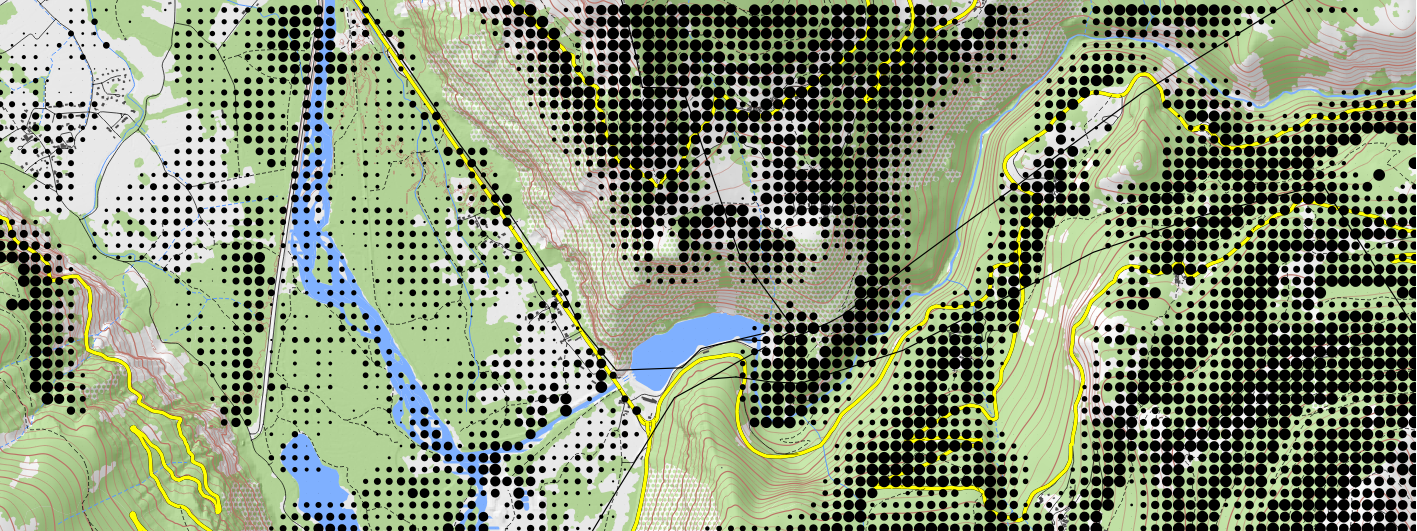
\includegraphics{../figures/ZLC_SousProche_Chemin/ZLC_SousProche_2.png}};
    \draw[-] ([yshift=-1cm]img1.south east) --++ (-1,0) node[et,pos=.5] {\SI{500}{\meter}};
    \draw[RdBu-9-1,thick,draw] (img1.south west) rectangle (img1.north east);
  \end{tikzpicture}
}
%
\begin{tikzpicture}[overlay, remember picture,RdBu-9-1,thick,draw,inner sep=0pt,outer sep=0pt]
  \draw (B1) -- (img1);
\end{tikzpicture}
